\documentclass[border=5pt]{standalone}
\usepackage[T1]{fontenc}
\usepackage{lmodern,amsmath}
\usepackage{tikz}
\usetikzlibrary{patterns,arrows.meta}
\begin{document}
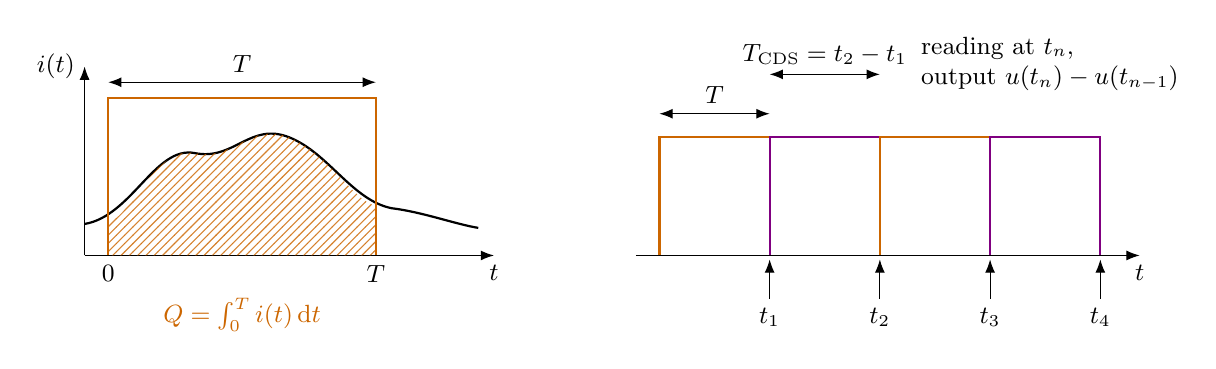
\begin{tikzpicture}[font=\small,>=Latex]
% left: one window
\begin{scope}
\draw[->] (0,0) -- (5.2,0) node[below]{$t$};
\draw[->] (0,0) -- (0,2.4) node[left]{$i(t)$};
\draw[thick] (0,0.4) .. controls (0.6,0.5) and (0.9,1.4) .. (1.4,1.3)
  .. controls (1.9,1.2) and (2.1,1.7) .. (2.6,1.5)
  .. controls (3.1,1.3) and (3.4,0.7) .. (3.9,0.6)
  .. controls (4.3,0.55) and (4.7,0.4) .. (5.0,0.35);
\fill[pattern=north east lines, pattern color=orange!80!black, opacity=.8]
  (0.3,0) -- (0.3,0.42) .. controls (0.6,0.5) and (0.9,1.4) .. (1.4,1.3)
  .. controls (1.9,1.2) and (2.1,1.7) .. (2.6,1.5)
  .. controls (3.1,1.3) and (3.4,0.7) .. (3.7,0.63) -- (3.7,0) -- cycle;
\draw[thick,orange!80!black] (0.3,0) -- (0.3,2.0) -- (3.7,2.0) -- (3.7,0);
\draw[<->] (0.3,2.2) -- (3.7,2.2) node[midway,above]{$T$};
\node[below] at (0.3,0) {$0$};
\node[below] at (3.7,0) {$T$};
\node[orange!80!black] at (2.0,-0.75) {$Q=\int_0^T i(t)\,\mathrm{d}t$};
\end{scope}
% right: frame sequence
\begin{scope}[xshift=7cm]
\draw[->] (0,0) -- (6.4,0) node[below]{$t$};
\foreach \k/\c in {0/orange!80!black,1/violet,2/orange!80!black,3/violet}{
  \draw[thick,\c] ({0.3+1.4*\k},0) -- ({0.3+1.4*\k},1.5) -- ({1.7+1.4*\k},1.5) -- ({1.7+1.4*\k},0);
}
\foreach \k in {1,2,3,4}{
  \draw[->] ({0.3+1.4*\k},-0.55) -- ({0.3+1.4*\k},-0.05);
  \node[below] at ({0.3+1.4*\k},-0.55) {$t_{\k}$};
}
\draw[<->] (0.3,1.8) -- (1.7,1.8) node[midway,above]{$T$};
\draw[<->] (1.7,2.3) -- (3.1,2.3) node[midway,above]{$T_{\rm CDS}=t_2-t_1$};
\node[align=left,anchor=north west] at (3.5,2.9) {reading at $t_n$,\\ output $u(t_n)-u(t_{n-1})$};
\end{scope}
\end{tikzpicture}
\end{document}
